\documentclass[11pt]{report}
\usepackage{./assignment}
\usepackage{graphicx}

\lecturenumber{2}       % assignment number
\duedate{13:00, April 12, 2018}

% Fill in your name and email address
\stuinfo{George Maratos, Ashwani Khemani}{gmarat2@uic.edu, akhema2@uic.edu}
\graphicspath{{./}{./Figures/}}

\begin{document}

\maketitle

\section*{Question P1}
\begin{verbatim}
iter func.val gap time feval.num train_lett_err train_word_err test_lett_err test_word_err
0 24.5949329 4.55704418 0.521893978 1 92.309174 100.000000 93.091357 100.000000
1 20.2619527 5.09500228 2.1071229 3 71.379031 100.000000 72.095711 100.000000
2 17.4280532 3.65686478 2.90276504 4 66.662814 99.825480 67.009594 99.883687
3 15.3063722 2.66873138 3.70153904 5 53.442762 97.643979 54.005317 97.702821
4 13.2139426 2.13033316 4.48281908 6 45.382037 96.160558 46.075598 95.347485
5 10.8951126 2.51806306 5.28561425 7 39.675567 91.826643 40.808384 92.294272
6 9.33821858 1.17139586 6.07544017 8 33.791855 87.056428 34.978615 87.699913
7 8.76213396 0.87446294 6.86494994 9 31.568605 84.293194 32.632066 85.228264
8 7.90650424 0.849892316 7.6622529 10 28.570878 80.424666 29.638192 81.942425
9 7.31265051 1.54717585 8.45745993 11 27.129812 77.370564 28.385928 78.016865
10 6.80867555 0.727934637 9.26300693 12 24.594459 73.007563 25.892960 74.498401
:
:
95 3.33946396 0.00445979302 76.2979987 98 10.858090 40.517743 14.499287 49.520209
Optimization converged with status CONVERGED_GTTOL.
\end{verbatim}

\section*{Question P2}
See figure 1 for the plot. Yes, using a larger value of $\lambda$
will allow for faster convergence.

\begin{figure}[b]
\centering
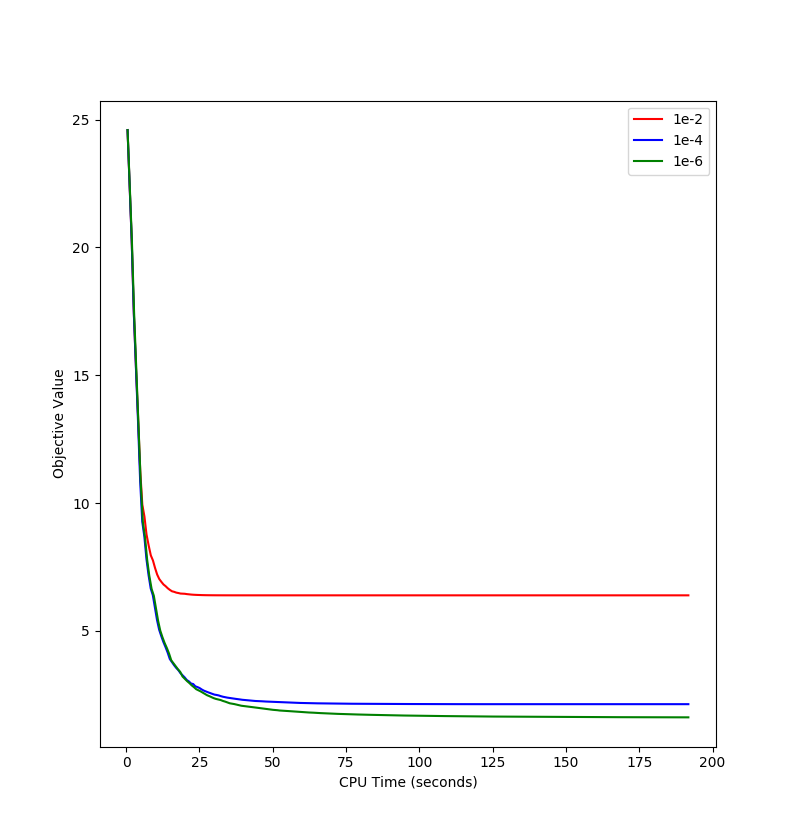
\includegraphics[scale=0.4]{p2_figure.png}
\caption{Determining the effect of lambda on Convergence Time}
\end{figure}
\section*{Question P3}
See figure 2 for the plot. We observe that while test error is
higer than train error, the model does a good job of generalizing
well for letter wise error. Word error is much higher in general,
but this is expected because getting the entire word correct is
much harder than getting a single letter. The objective value 
drops dramaticaly during training for the first 20 seconds. We
conclude that a drop in objective value is correlated with a drop
in error, because we observe a similar drop in the same time frame.


\begin{figure}[b]
\centering
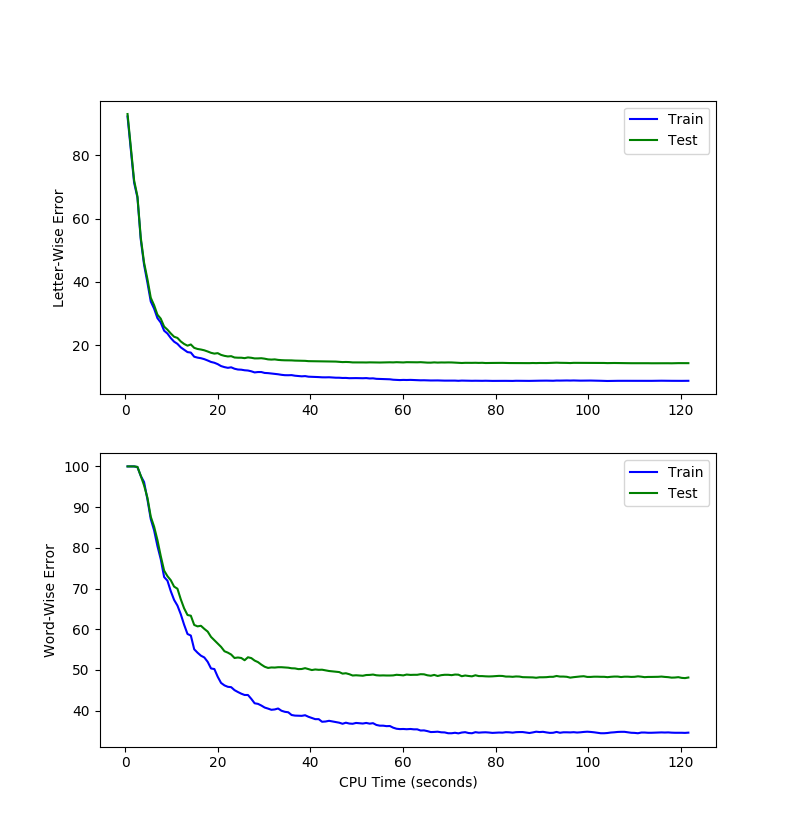
\includegraphics[scale=0.4]{p3_figure.png}
\caption{Plot of Letter and Word Error}
\end{figure}

\section*{Question P4}
See figure 3 for the plot. The curve is not linear, as can be observed
in the plot. Linearity breaks around 5 cores. We cannot expect a perpetual
linear speed up from increased levels of parallelization. Consider an
arbitrary task that has 100 independent atomic operations. Parallelizing
this task will speed up the task, but there will be no benefit from going
to 101 cores from 100 because the last core will remain idle and contribute
nothing.

\begin{figure}[b]
\centering
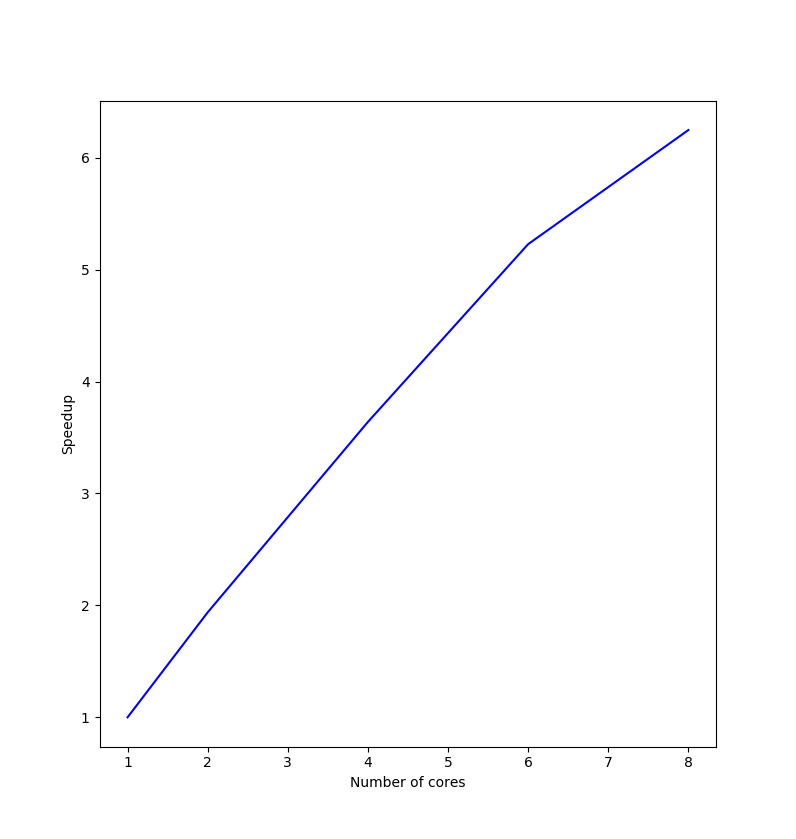
\includegraphics[scale=0.4]{p4_figure.png}
\caption{Plot of Letter and Word Error}
\end{figure}

\section*{Question P5}
No we do not need to store $C_{train}$. We can instead, distribute $X_{train}$
and modify $loss\_coef$ to compute $g_{node}$ directly. This would allow us to
forget about $C_{train}$ entirely. The computational performance will not be 
significantly affected.

\end{document}
